\documentclass{article}\usepackage[]{graphicx}\usepackage[]{xcolor}
% maxwidth is the original width if it is less than linewidth
% otherwise use linewidth (to make sure the graphics do not exceed the margin)
\makeatletter
\def\maxwidth{ %
  \ifdim\Gin@nat@width>\linewidth
    \linewidth
  \else
    \Gin@nat@width
  \fi
}
\makeatother

\definecolor{fgcolor}{rgb}{0.345, 0.345, 0.345}
\newcommand{\hlnum}[1]{\textcolor[rgb]{0.686,0.059,0.569}{#1}}%
\newcommand{\hlsng}[1]{\textcolor[rgb]{0.192,0.494,0.8}{#1}}%
\newcommand{\hlcom}[1]{\textcolor[rgb]{0.678,0.584,0.686}{\textit{#1}}}%
\newcommand{\hlopt}[1]{\textcolor[rgb]{0,0,0}{#1}}%
\newcommand{\hldef}[1]{\textcolor[rgb]{0.345,0.345,0.345}{#1}}%
\newcommand{\hlkwa}[1]{\textcolor[rgb]{0.161,0.373,0.58}{\textbf{#1}}}%
\newcommand{\hlkwb}[1]{\textcolor[rgb]{0.69,0.353,0.396}{#1}}%
\newcommand{\hlkwc}[1]{\textcolor[rgb]{0.333,0.667,0.333}{#1}}%
\newcommand{\hlkwd}[1]{\textcolor[rgb]{0.737,0.353,0.396}{\textbf{#1}}}%
\let\hlipl\hlkwb

\usepackage{framed}
\makeatletter
\newenvironment{kframe}{%
 \def\at@end@of@kframe{}%
 \ifinner\ifhmode%
  \def\at@end@of@kframe{\end{minipage}}%
  \begin{minipage}{\columnwidth}%
 \fi\fi%
 \def\FrameCommand##1{\hskip\@totalleftmargin \hskip-\fboxsep
 \colorbox{shadecolor}{##1}\hskip-\fboxsep
     % There is no \\@totalrightmargin, so:
     \hskip-\linewidth \hskip-\@totalleftmargin \hskip\columnwidth}%
 \MakeFramed {\advance\hsize-\width
   \@totalleftmargin\z@ \linewidth\hsize
   \@setminipage}}%
 {\par\unskip\endMakeFramed%
 \at@end@of@kframe}
\makeatother

\definecolor{shadecolor}{rgb}{.97, .97, .97}
\definecolor{messagecolor}{rgb}{0, 0, 0}
\definecolor{warningcolor}{rgb}{1, 0, 1}
\definecolor{errorcolor}{rgb}{1, 0, 0}
\newenvironment{knitrout}{}{} % an empty environment to be redefined in TeX

\usepackage{alltt}
\usepackage{amsmath} %This allows me to use the align functionality.
                     %If you find yourself trying to replicate
                     %something you found online, ensure you're
                     %loading the necessary packages!
\usepackage{amsfonts}%Math font
\usepackage{graphicx}%For including graphics
\usepackage{hyperref}%For Hyperlinks
\usepackage[shortlabels]{enumitem}% For enumerated lists with labels specified
                                  % We had to run tlmgr_install("enumitem") in R
\hypersetup{colorlinks = true,citecolor=black} %set citations to have black (not green) color
\usepackage{natbib}        %For the bibliography
\setlength{\bibsep}{0pt plus 0.3ex}
\bibliographystyle{apalike}%For the bibliography
\usepackage[margin=0.50in]{geometry}
\usepackage{float}
\usepackage{multicol}

%fix for figures
\usepackage{caption}
\newenvironment{Figure}
  {\par\medskip\noindent\minipage{\linewidth}}
  {\endminipage\par\medskip}
\IfFileExists{upquote.sty}{\usepackage{upquote}}{}
\begin{document}

\vspace{-1in}
\title{Lab 10 -- MATH 240 -- Computational Statistics}

\author{
  Jack Schaeffer \\
  Professor Cipolli  \\
  Math 240  \\
  {\tt jschaeffer@colgate.edu}
}

\date{April 8, 2025}

\maketitle

\begin{multicols}{2}
%\raggedcolumns % If your spacing gets messed up try uncommenting 
                % this line
\begin{abstract}

Focused on analyzing effects on the margin of error, we calculated differing approximate margins of errors based on Gallup polls. We first determined how this value changes based on sample size before comparing the effect within a binomial distribution in comparison to sample size and p.
\end{abstract}

\noindent \textbf{Keywords:} Binomial distribution, margin of error, resampling

\section{Introduction}

Questions concerning margin of error stemmed from the Gallup polls article "\textit{How Are Polls Conducted?}'' that described the formation of polls and how statistical calculations are made. The article asserted that doubling their 1000 person sample size would serve to halve the margin of error, and my work was testing this with my own calculations. My initial work was testing margin of error after doubling sample size of a known p value before moving on to compare these values with resampling of the Gallup polls data. The final test on margin of error was comparing the margin of error of varying sample size and p values through both simulations of the binomial distribution and calculation of the Wilson Estimate.

\section{Methods}

My work was mainly focused on simulating or estimating data that could then be summarized with \texttt{tidyverse} to obtain more useful information \citep{tidyverse}. To first answer the question of doubling sample size, I ran two separate simulations of the binomial distribution under the assumption that Gallup polls produced an accurate p value. Although I could not use resampling to test a larger sample size than the given 1004, resampling was an effective way to compare the simulated margin of error to ensure that the given p value is a reasonable assumption. 

I tested the margin of error over numerous combinations of sample size and p value in the same way as my initial simulations, but scaled to include far more combinations of p and n values. I used a similar combination fo p and n values to test the margin of error calculated through the Wilson Estimate, so that I could compare the effect of sample size and p value on margin of error through both methods.

\section{Results}


\begin{figure}[H]
 \begin{center}
 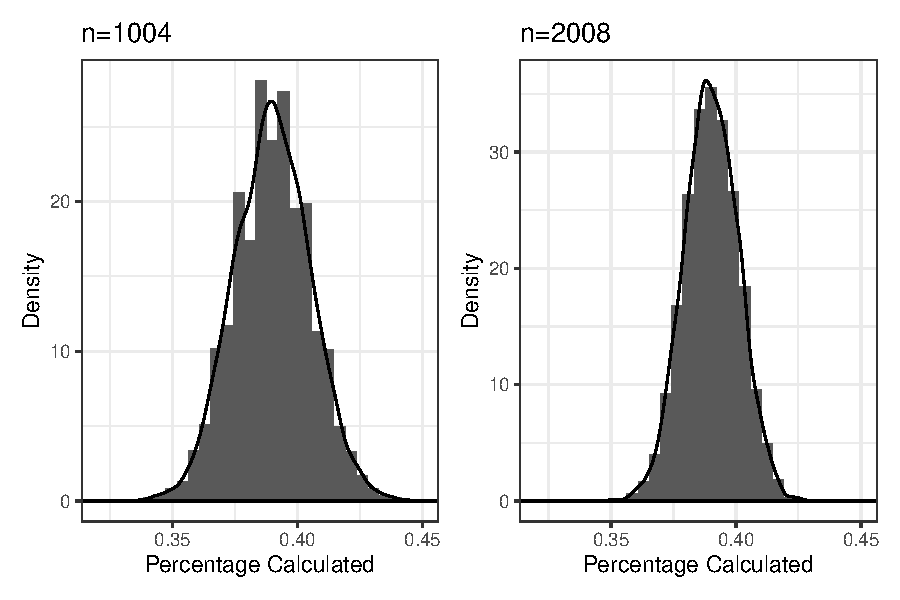
\includegraphics[scale=0.65]{part1_comparison.pdf}
 \caption{A comparison of simulations for different sample sizes}
 \label{plot1}
 \end{center}
 \end{figure}


\begin{figure}[H]
 \begin{center}
 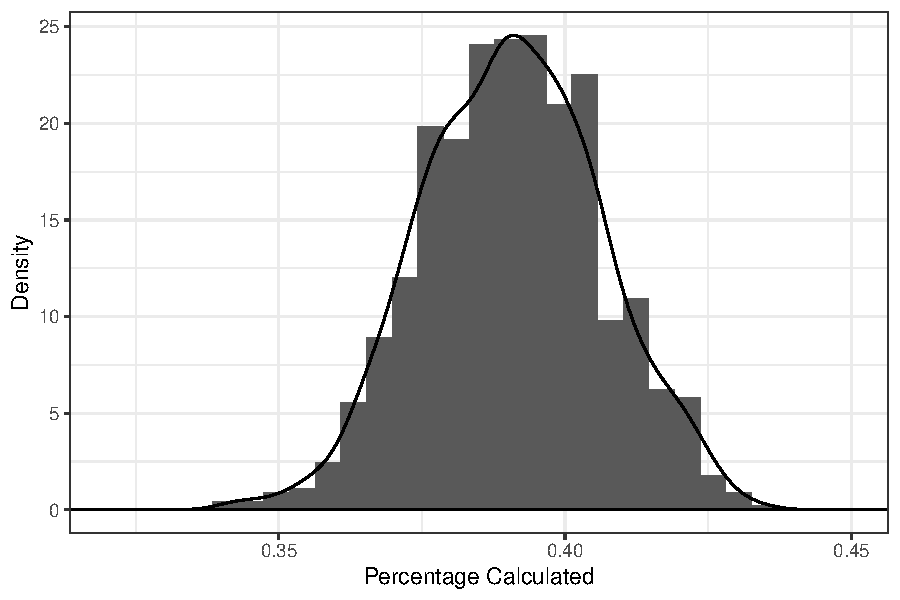
\includegraphics[scale=0.45]{resample_plot.pdf}
 \caption{Calculated p values with resampling}
 \label{plot2}
 \end{center}
 \end{figure}

\begin{figure}[H]
 \begin{center}
 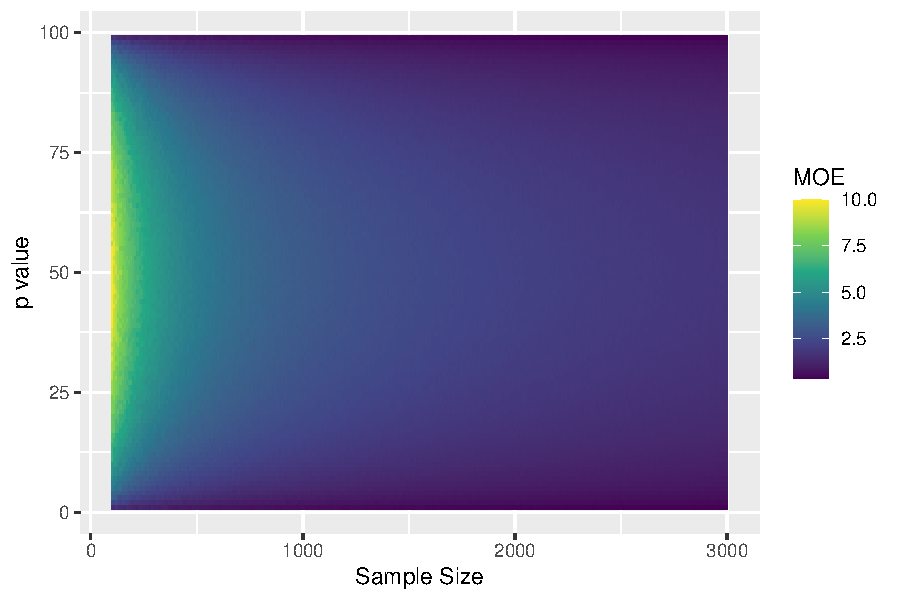
\includegraphics[scale=0.6]{sim_moe.pdf}
 \caption{Simulated margin of error for binomial distribution}
 \label{plot3}
 \end{center}
 \end{figure}

\begin{figure}[H]
 \begin{center}
 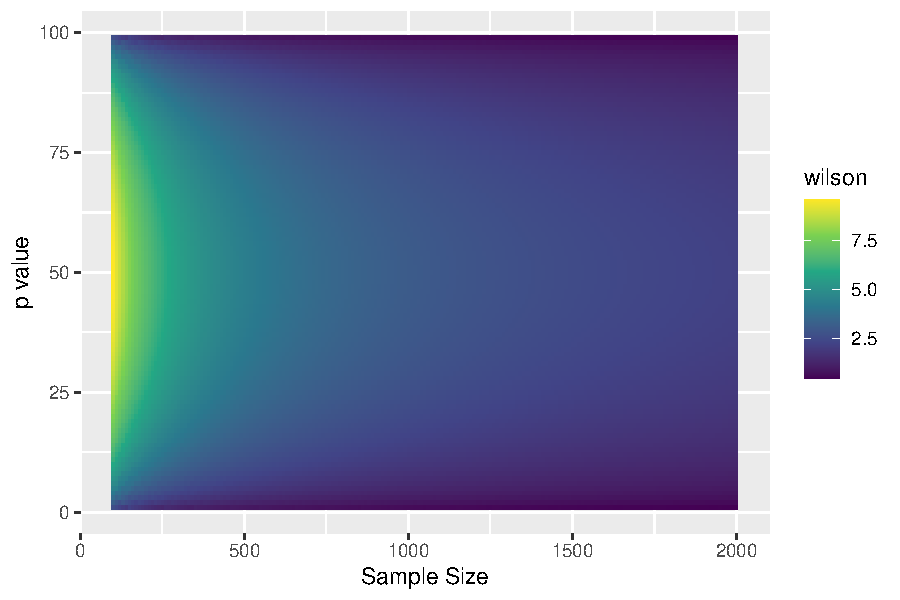
\includegraphics[scale=0.6]{wilson_moe.pdf}
 \caption{Margin of error calculated through Wilson Estimate}
 \label{plot4}
 \end{center}
 \end{figure}




Tie together the Introduction -- where you introduce the problem at hand -- and the methods --  what you propose to do to answer the question. Present your data, the results of your analyses, and how each reported aspect contributes to answering the question. This section should include table(s), statistic(s), and graphical displays. Make sure to put the results in a sensible order and that each result contributes a logical and developed solution. It should not just be a list. Avoid being repetitive. 

\subsection{Results Subsection}
Subsections can be helpful for the Results section, too. This can be particularly helpful if you have different questions to answer. 


\section{Discussion}
 You should objectively evaluate the evidence you found in the data. Do not embellish or wish-terpet (my made-up phase for making an interpretation you, or the researcher, wants to be true without the data \emph{actually} supporting it). Connect your findings to the existing information you provided in the Introduction.

Finally, provide some concluding remarks that tie together the entire paper. Think of the last part of the results as abstract-like. Tell the reader what they just consumed -- what's the takeaway message?

%%%%%%%%%%%%%%%%%%%%%%%%%%%%%%%%%%%%%%%%%%%%%%%%%%%%%%%%%%%%%%%%%%%%%%%%%%%%%%%%
% Bibliography
%%%%%%%%%%%%%%%%%%%%%%%%%%%%%%%%%%%%%%%%%%%%%%%%%%%%%%%%%%%%%%%%%%%%%%%%%%%%%%%%
\vspace{2em}


\begin{tiny}
\bibliography{bib}
\end{tiny}
\end{multicols}

%%%%%%%%%%%%%%%%%%%%%%%%%%%%%%%%%%%%%%%%%%%%%%%%%%%%%%%%%%%%%%%%%%%%%%%%%%%%%%%%
% Appendix
%%%%%%%%%%%%%%%%%%%%%%%%%%%%%%%%%%%%%%%%%%%%%%%%%%%%%%%%%%%%%%%%%%%%%%%%%%%%%%%%

\end{document}
